\documentclass[xcolor=svgnames]{beamer}\usepackage[]{graphicx}\usepackage[]{color}
%% maxwidth is the original width if it is less than linewidth
%% otherwise use linewidth (to make sure the graphics do not exceed the margin)
\makeatletter
\def\maxwidth{ %
  \ifdim\Gin@nat@width>\linewidth
    \linewidth
  \else
    \Gin@nat@width
  \fi
}
\makeatother

\definecolor{fgcolor}{rgb}{0.345, 0.345, 0.345}
\newcommand{\hlnum}[1]{\textcolor[rgb]{0.686,0.059,0.569}{#1}}%
\newcommand{\hlstr}[1]{\textcolor[rgb]{0.192,0.494,0.8}{#1}}%
\newcommand{\hlcom}[1]{\textcolor[rgb]{0.678,0.584,0.686}{\textit{#1}}}%
\newcommand{\hlopt}[1]{\textcolor[rgb]{0,0,0}{#1}}%
\newcommand{\hlstd}[1]{\textcolor[rgb]{0.345,0.345,0.345}{#1}}%
\newcommand{\hlkwa}[1]{\textcolor[rgb]{0.161,0.373,0.58}{\textbf{#1}}}%
\newcommand{\hlkwb}[1]{\textcolor[rgb]{0.69,0.353,0.396}{#1}}%
\newcommand{\hlkwc}[1]{\textcolor[rgb]{0.333,0.667,0.333}{#1}}%
\newcommand{\hlkwd}[1]{\textcolor[rgb]{0.737,0.353,0.396}{\textbf{#1}}}%

\usepackage{framed}
\makeatletter
\newenvironment{kframe}{%
 \def\at@end@of@kframe{}%
 \ifinner\ifhmode%
  \def\at@end@of@kframe{\end{minipage}}%
  \begin{minipage}{\columnwidth}%
 \fi\fi%
 \def\FrameCommand##1{\hskip\@totalleftmargin \hskip-\fboxsep
 \colorbox{shadecolor}{##1}\hskip-\fboxsep
     % There is no \\@totalrightmargin, so:
     \hskip-\linewidth \hskip-\@totalleftmargin \hskip\columnwidth}%
 \MakeFramed {\advance\hsize-\width
   \@totalleftmargin\z@ \linewidth\hsize
   \@setminipage}}%
 {\par\unskip\endMakeFramed%
 \at@end@of@kframe}
\makeatother

\definecolor{shadecolor}{rgb}{.97, .97, .97}
\definecolor{messagecolor}{rgb}{0, 0, 0}
\definecolor{warningcolor}{rgb}{1, 0, 1}
\definecolor{errorcolor}{rgb}{1, 0, 0}
\newenvironment{knitrout}{}{} % an empty environment to be redefined in TeX

\usepackage{alltt}
\usetheme{Boadilla}
\usecolortheme[named=SeaGreen]{structure}
\usepackage{graphicx}
\usepackage{breqn}
\usepackage{xcolor}
\usepackage{booktabs}
\usepackage{verbatim}
\usepackage{tikz}
\usepackage{lmodern}
\usetikzlibrary{shadows,arrows,positioning}
\definecolor{links}{HTML}{2A1B81}
\hypersetup{colorlinks,linkcolor=links,urlcolor=links}
\usepackage{pgfpages}

\tikzstyle{block} = [rectangle, draw, text width=9em, text centered, rounded corners, minimum height=3em, minimum width=7em, top color = white, bottom color=brown!30,  drop shadow]

\newcommand{\ShowSexpr}[1]{\texttt{{\char`\\}Sexpr\{#1\}}}

\newcommand{\Bigtxt}[1]{\textbf{\textit{#1}}}
\IfFileExists{upquote.sty}{\usepackage{upquote}}{}
\begin{document}

\title[Overview of SWMP and retrieval]{SWMP data retrieval and preparation}

\author[M. Beck, T. O'Brien]{Marcus W. Beck\inst{1} \and Todd D. O'Brien\inst{2}}

\date{}

\institute[]{\inst{1} ORISE, USEPA NHEERL Gulf Ecology Division\\ Email: \href{mailto:beck.marcus@epa.gov}{beck.marcus@epa.gov} \and \inst{2} NOAA/NMFS Copepod Project\\ Email: \href{todd.obrien@noaa.gov}{todd.obrien@noaa.gov}}

% knitr setup


% load SWMPr from local


%%%%%%
\begin{frame}
\vspace{0.3in}
\centerline{
\begin{tikzpicture}
  \node[drop shadow={shadow xshift=0ex,shadow yshift=0ex},fill=white,draw] at (0,0) {
\includegraphics[width=0.9\textwidth]{bg_main.jpg}};
\end{tikzpicture}}
\titlepage
\end{frame}

%%%%%%
\begin{frame}{Objectives and agenda}
\begin{itemize}
\onslide<+->
\item Objectives \\~\\
\begin{itemize}
\item What are the various ways data are obtained from SWMP? \\~\\
\item What are some issues that need to be addressed before importing into a statistical program to conduct a time series analysis? \\~\\
\end{itemize}
\onslide<+->
\item Agenda \\~\\
\begin{itemize}
\item Brief overview of SWMP network and available data \\~\\
\item Format and potential issues with output data \\~\\
\item Retrieving and importing the data \\~\\
\end{itemize}
\end{itemize}
\end{frame}

%%%%%%
\begin{frame}{Interactive portion}
You can follow along later in this module: \\~\\
\begin{itemize}
\item dataset1\\~\\
\item script1 \\~\\
\end{itemize}
\Large
\centerline{\emph{Interactive! Interrupt me!}}
\end{frame}

%%%%%%
\begin{frame}{Overview of SWMP and available data}
SWMP - System Wide Monitoring Program, initiated in 1995 to provide continuous monitoring data at over 300 stations in 28 US estuaries \\~\\
\centerline{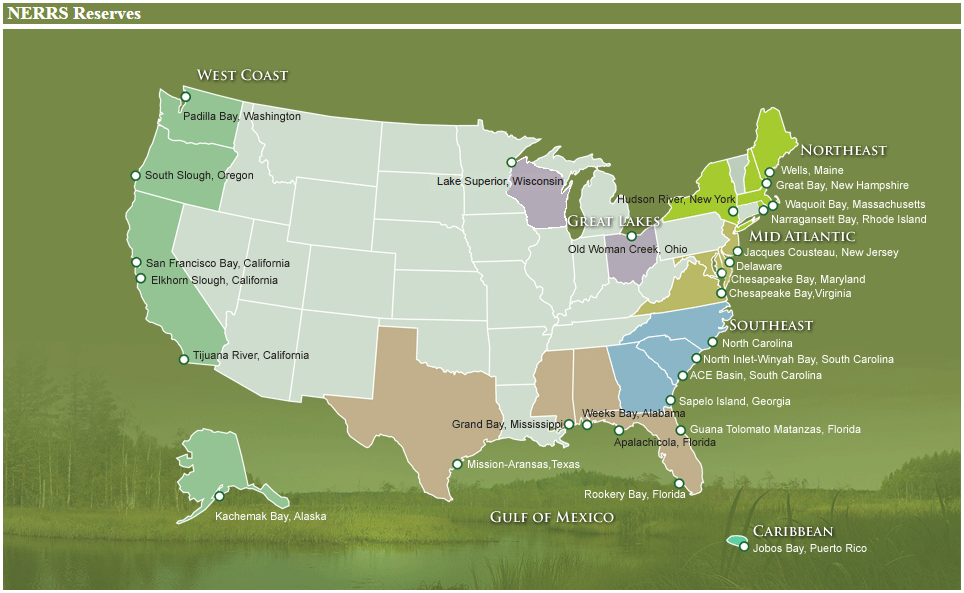
\includegraphics[width = 0.8\textwidth]{NERRS_locations.png}}
\tiny
\flushright
\href{http://nerrs.noaa.gov/ReservesMap.aspx}{http://nerrs.noaa.gov/ReservesMap.aspx}
\end{frame}

%%%%%%
\begin{frame}[t]{Overview of SWMP and available data}
CDMO is your one-stop shop for retrieving SWMP data \\~\\
\centerline{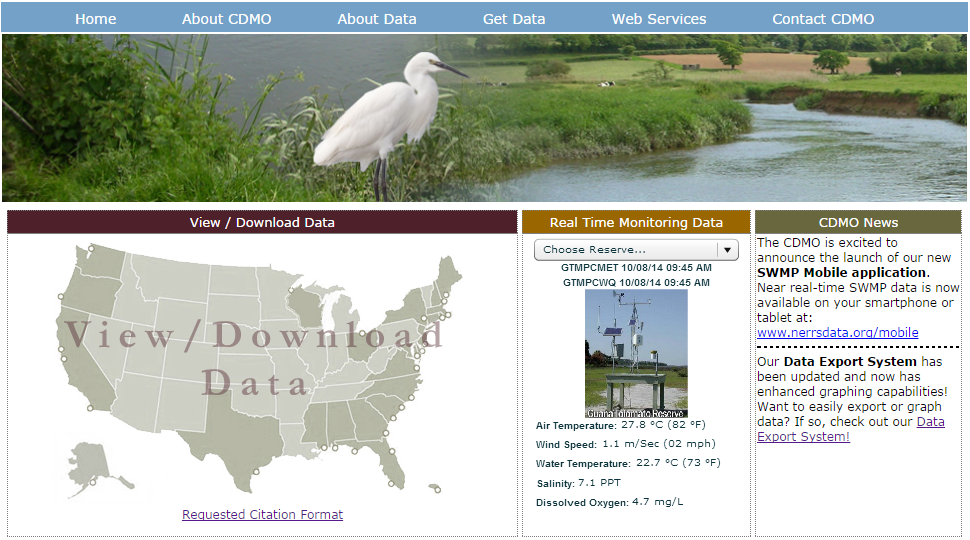
\includegraphics[width = \textwidth]{cdmo_front.png}}
\end{frame}

%%%%%%
\begin{frame}{Overview of SWMP and available data}
Data can be exported from CDMO \href{http://cdmo.baruch.sc.edu/get/landing.cfm}{several ways}:\\~\\
\centerline{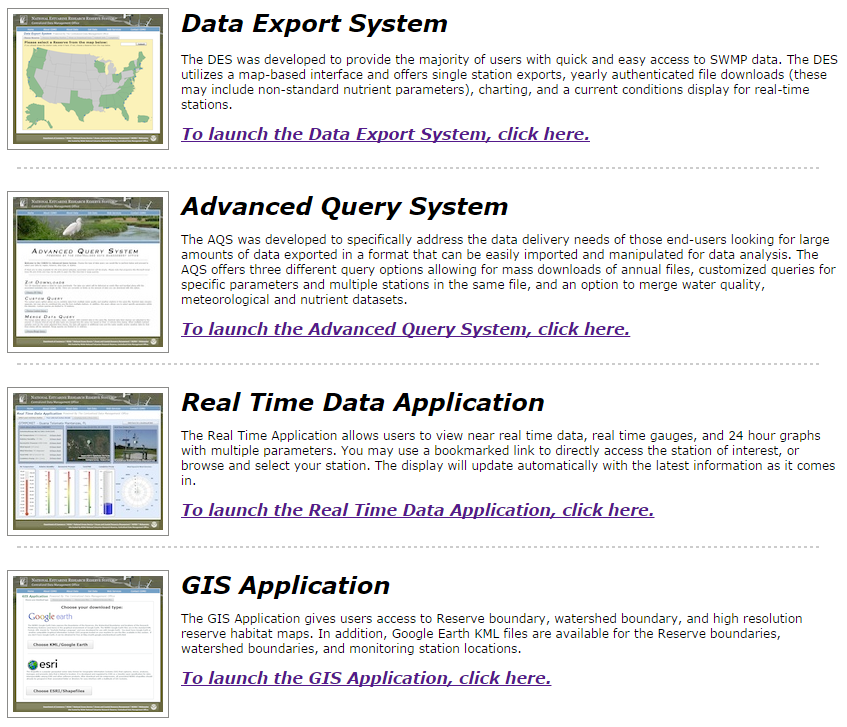
\includegraphics[width = 0.6\textwidth]{get_data.png}}
\end{frame}

%%%%%%
\begin{frame}{Overview of SWMP and avialable data}
You can also use the \href{https://github.com/fawda123/SWMPr}{SWMPr} package to retrieve data \\~\\
Data retrieval functions connect to the CDMO \href{http://cdmo.baruch.sc.edu/webservices.cfm}{web services}, more about this later \\~\\
\centerline{
\includegraphics[width = 0.8\textwidth]{web_serv.png}}
\end{frame}

%%%%%%
\begin{frame}{Overview of SWMP and available data}
A wide range of data can be requested... a few records for one site to all records for multiple sites \\~\\
Requests can return a lot of data so make sure you have clear objectives \\~\\
Check the \href{http://cdmo.baruch.sc.edu/data/availableOne.cfm}{available data} before making a request! \\~\\
\begin{itemize}
\item station names \\~\\
\item data types \\~\\
\item date ranges \\~\\
\item parameters \\~\\
\end{itemize}
\end{frame}

%%%%%%
\begin{frame}[t]{Overview of SWMP and available data}
Available data: \href{http://cdmo.baruch.sc.edu/data/availableOne.cfm}{http://cdmo.baruch.sc.edu/data/availableOne.cfm}\\~\\
\centerline{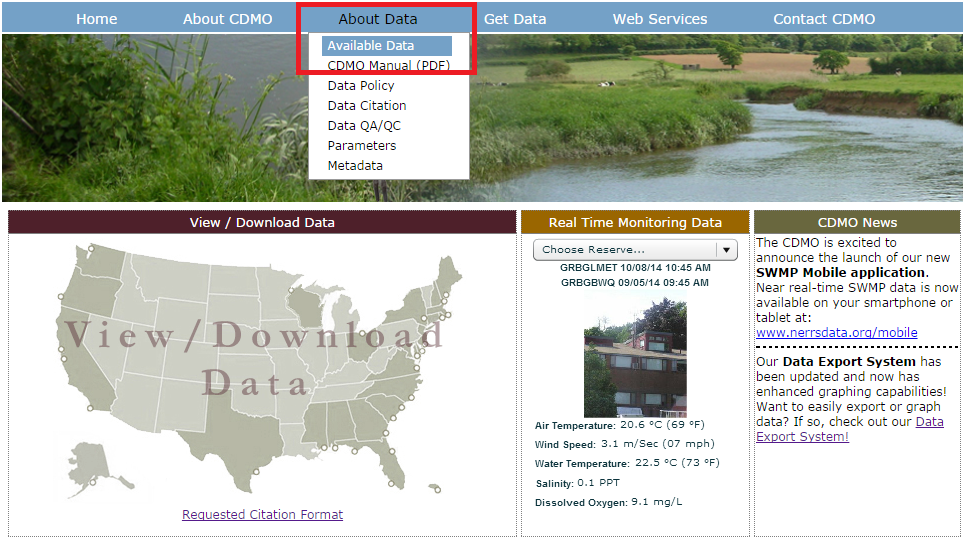
\includegraphics[width = 0.9\textwidth]{avail_dat2.png}}
\end{frame}

%%%%%%
\begin{frame}{Overview of SWMP and available data}
\onslide<+->
How to view available data:\\~\\
\begin{itemize}
\item Trial-and-error (not recommended) \\~\\
\item View online: \href{http://cdmo.baruch.sc.edu/data/availableOne.cfm}{http://cdmo.baruch.sc.edu/data/availableOne.cfm}  \\~\\
\item View after request: `sampling_stations.csv'  \\~\\
\item View after request: year and station specific .doc file  \\~\\
\item Retrieve from within R (will cover later) \\~\\
\end{itemize}
\onslide<+->
\centerline{\emph{Now that you have the data, what do they look like?}} 
\end{frame}

%%%%%%
\begin{frame}{Format and potential issues with output data}
\onslide<+->
To orient yourself, understand the NERRS/SWMP naming convention\\~\\
\Bigtxt{Site} (reserve), \Bigtxt{station}, and \Bigtxt{parameter type} are identified by a 7 or 8 character name \\~\\
\onslide<+->
E.g., elkcwmet \\~\\
\onslide<+->
\begin{itemize}
\item elk: site, Elkhorn Slough \\~\\
\item cw: station, Caspian Weather Station \\~\\
\item met: parameter type (weather)
\end{itemize}
\end{frame}

%%%%%%
\begin{frame}{Format and potential issues with output data}
\onslide<+->
The fundamental unit of data is the `station' defined by a parameter type \\~\\
The parameters for a station are specific to the parameter type \\~\\
\onslide<+->
\begin{columns}[t]
\begin{column}{0.3\textwidth}
\Bigtxt{Nutrients} \\~\\
po4f, chla\_n, no3f, no2f, nh4f, no23f, ke\_n, urea
\end{column}
\begin{column}{0.3\textwidth}
\Bigtxt{Water quality} \\~\\
temp, spcond, sal, do\_pct, do\_mgl, depth, cdepth, level, clevel, ph, turb, chlfluor
\end{column}
\begin{column}{0.3\textwidth}
\Bigtxt{Meteorology} \\~\\
atemp, rh, bp, wspd, maxwspd, wdir, sdwdir, totpar, totprcp, cumprcp, totsorad \\~\\
\end{column}
\end{columns}
\end{frame}

%%%%%%
\begin{frame}{Format and potential issues with output data}
Each parameter will also have a QAQC column, with the prefix `f\_' \\~\\
E.g., `atemp' and `f\_atemp' \\~\\
Values in these columns describe whether the data passed automated QAQC checks \\~\\
\centerline{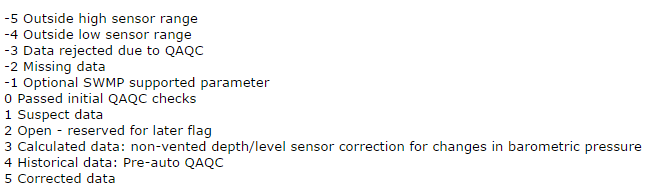
\includegraphics[width = 0.9\textwidth]{qaqc_flags.png}}
\end{frame}

%%%%%%
\begin{frame}{Format and potential issues with output data}
You will have to decide how to handle QAQC...\\~\\
\centerline{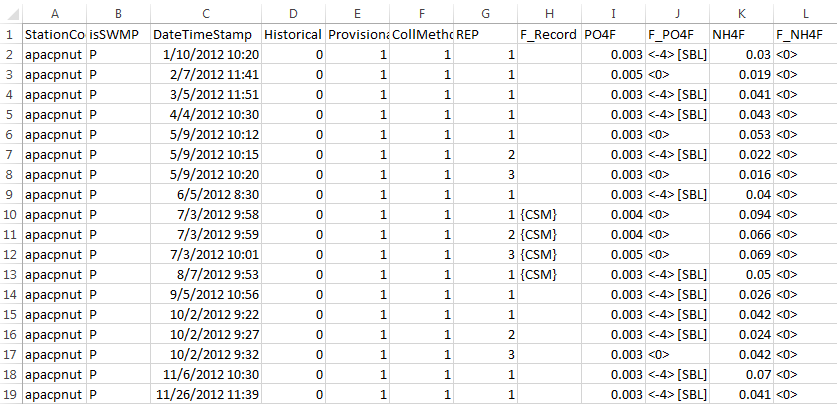
\includegraphics[width = 0.8\textwidth]{qaqc_ex.png}}
\vspace{0.2in}
CDMO has limited export options for dealing with bad QAQC flags \\~\\
We will learn how to handle QAQC flags in R
\end{frame}

%%%%%%
\begin{frame}{Format and potential issues with output data}
The final piece of of the puzzle is the DateTimeStamp \\~\\
Format is month/day/year hours:minutes, based on UTC offset and no daylight savings!\\~\\
Varies by station and parameter type \\~\\
\begin{columns}[t]
\begin{column}{0.4\textwidth}
\centerline{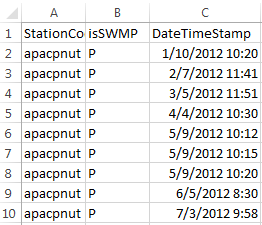
\includegraphics[width = 0.9\textwidth]{timestamp_ex1.png}}
\end{column}
\begin{column}{0.4\textwidth}
\centerline{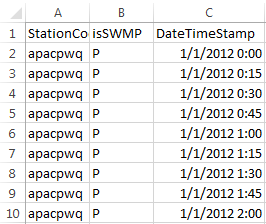
\includegraphics[width = 0.9\textwidth]{timestamp_ex2.png}}
\end{column}
\end{columns}
\end{frame}

%%%%%%
\begin{frame}{Format and potential issues with output data}
\onslide<+->
What are the challenges for evaluating SWMP data?? \\~\\
\onslide<+->
\begin{itemize}
\item Knowing what we want (I can't help with this) \\~\\
\onslide<+->
\item Dealing with QAQC columns and removing `bad' observations \\~\\
\onslide<+->
\item Data we don't want... extra columns or irrelevant parameters \\~\\
\onslide<+->
\item Combining data for comparison
\onslide<+-> 
\item Issues inherent with time series, e.g., missing data
\end{itemize}
\onslide<+->
\centerline{\emph{We will learn how to handle most of these challenges!}}
\end{frame}

%%%%%%
\begin{frame}{Overview of the SWMPr package}
\onslide<+->
\textbf{\emph{What}}: An R package for retrieving, organizing and analyzing SWMP data \\~\\
\onslide<+->
\Bigtxt{Why}: There are many challenges for working with SWMP data... a toolkit for addressing these challenges using an open-source format will be useful (I hope!) \\~\\
\onslide<+->
\Bigtxt{How}: \\~\\
\begin{itemize}
\item Install R/RStudio on your computer (done already?) \\~\\
\item Install the SWMPr package \\~\\
\item Use the SWMPr functions to \Bigtxt{retrieve}, \Bigtxt{organize}, and \Bigtxt{analyze} SWMP data 
\end{itemize}
\end{frame}

%%%%%%
\begin{frame}{Overview of the SWMPr package}
This is where SWMPr lives - \href{https://github.com/fawda123/SWMPr}{https://github.com/fawda123/SWMPr}\\~\\
\centerline{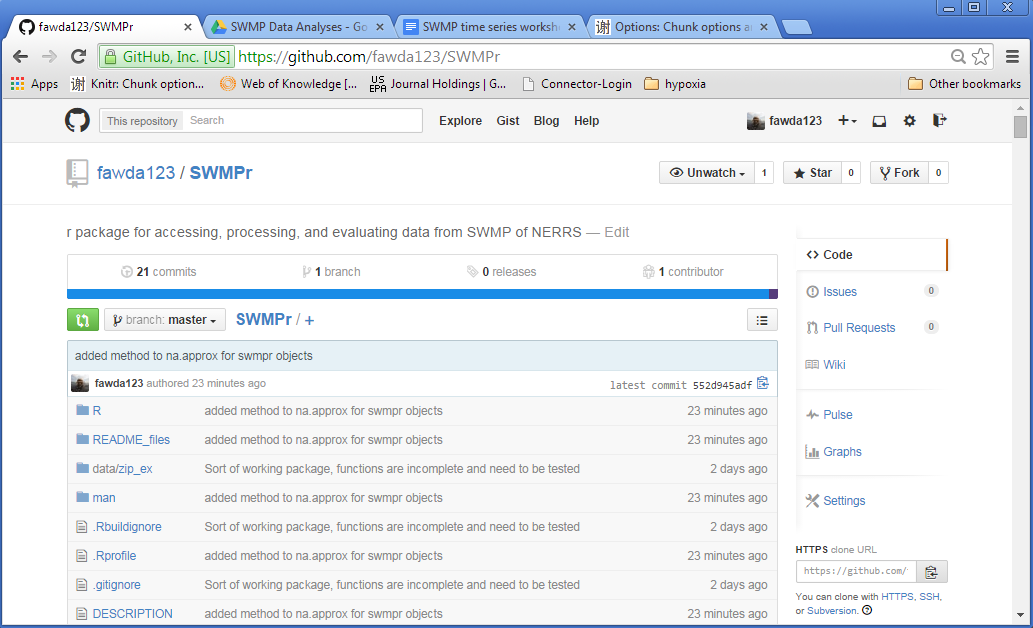
\includegraphics[width = 0.9\textwidth]{swmpr_github.png}}
\end{frame}

%%%%%%
\begin{frame}{Overview of the SWMPr package}
Scroll down the page to view the \href{https://github.com/fawda123/SWMPr/blob/master/README.md}{README} file, all instructions here...\\~\\
\centerline{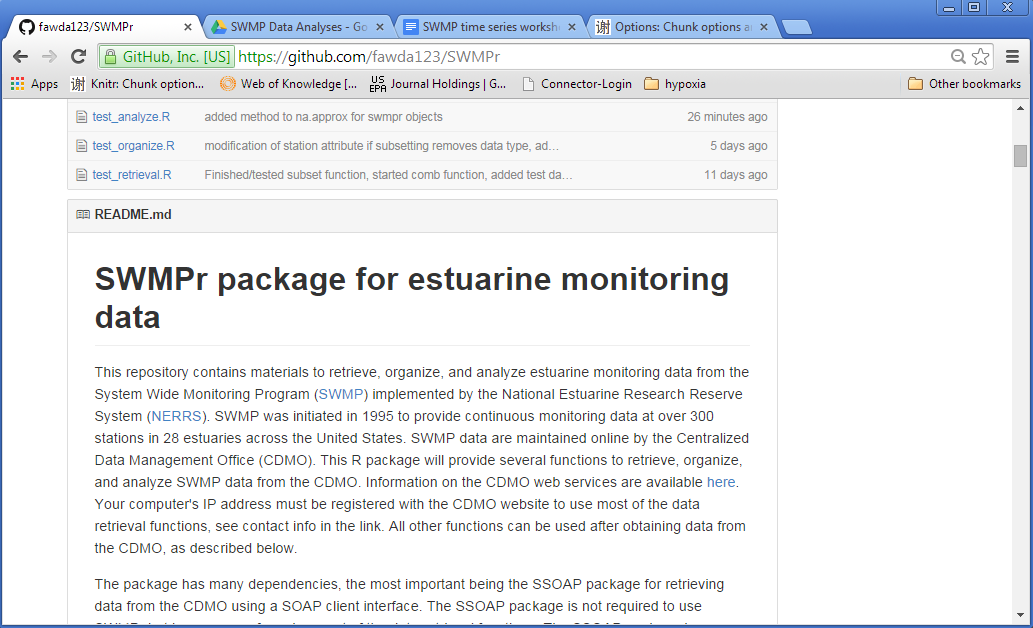
\includegraphics[width = 0.9\textwidth]{swmpr_readme.png}}
\end{frame}

%%%%%%
\begin{frame}[t, fragile]{Overview of the SWMPr package}
Installation instructions are in the \href{https://github.com/fawda123/SWMPr/blob/master/README.md}{README} \\~\\
Run these four lines to install the package
\begin{knitrout}
\definecolor{shadecolor}{rgb}{0.969, 0.969, 0.969}\color{fgcolor}\begin{kframe}
\begin{alltt}
\hlkwd{install.packages}\hlstd{(}\hlstr{'devtools'}\hlstd{)}
\hlkwd{library}\hlstd{(devtools)}
\hlkwd{install_github}\hlstd{(}\hlstr{'fawda123/SWMPr'}\hlstd{)}
\hlkwd{library}\hlstd{(SWMPr)}
\end{alltt}
\end{kframe}
\end{knitrout}
What is it doing? \\~\\
Packages can be installed from Github using the `install\_github' function from the devtools package
\end{frame}

%%%%%%
\begin{frame}[t, fragile]{Overview of the SWMPr package}
Your R console should look like this...\\~\\
\centerline{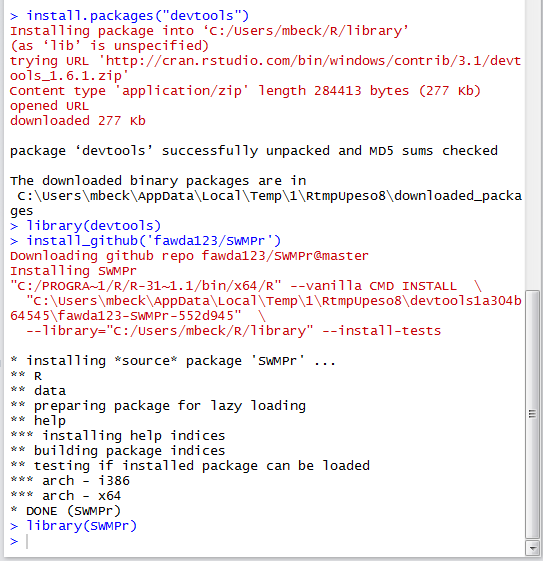
\includegraphics[width = 0.55\textwidth]{swmpr_install.png}}
\end{frame}

%%%%%%
\begin{frame}[fragile]{Overview of the SWMPr package}
What is provided in the SWMPr package? \\~\\
\begin{columns}[t]
\begin{column}{0.3\textwidth}
\Bigtxt{Retrieve}
\begin{knitrout}
\definecolor{shadecolor}{rgb}{0.969, 0.969, 0.969}\color{fgcolor}\begin{kframe}
\begin{alltt}
\hlstd{all_params}
\hlstd{all_params_dtrng}
\hlstd{single_param}
\hlstd{import_local}
\end{alltt}
\end{kframe}
\end{knitrout}
\end{column}
\begin{column}{0.3\textwidth}
\Bigtxt{Organize}
\begin{knitrout}
\definecolor{shadecolor}{rgb}{0.969, 0.969, 0.969}\color{fgcolor}\begin{kframe}
\begin{alltt}
\hlstd{qaqc.swmpr}
\hlstd{subset.swmpr}
\hlstd{setstep.swmpr}
\hlstd{comb.swmpr}
\end{alltt}
\end{kframe}
\end{knitrout}
\end{column}
\begin{column}{0.3\textwidth}
\Bigtxt{Analyze}
\begin{knitrout}
\definecolor{shadecolor}{rgb}{0.969, 0.969, 0.969}\color{fgcolor}\begin{kframe}
\begin{alltt}
\hlstd{aggregate.swmpr}
\hlstd{smoother.swmpr}
\hlstd{na.approx.swmpr}
\hlstd{plot.swmpr}
\hlstd{hist.swmpr}
\hlstd{lines.swmpr}
\hlstd{decomp.swmpr}
\end{alltt}
\end{kframe}
\end{knitrout}
\end{column}
\end{columns}
\vspace{0.15in}
Built around the concept of \Bigtxt{object-oriented programming} - retrieval functions return a data type with specific methods to organize and analyze
\end{frame}

%%%%%%
\begin{frame}[fragile]{Overview of the SWMPr package}
To view the help file for any function (including examples):
\begin{knitrout}
\definecolor{shadecolor}{rgb}{0.969, 0.969, 0.969}\color{fgcolor}\begin{kframe}
\begin{alltt}
\hlopt{?}\hlstd{all_params}
\end{alltt}
\end{kframe}
\end{knitrout}
\centerline{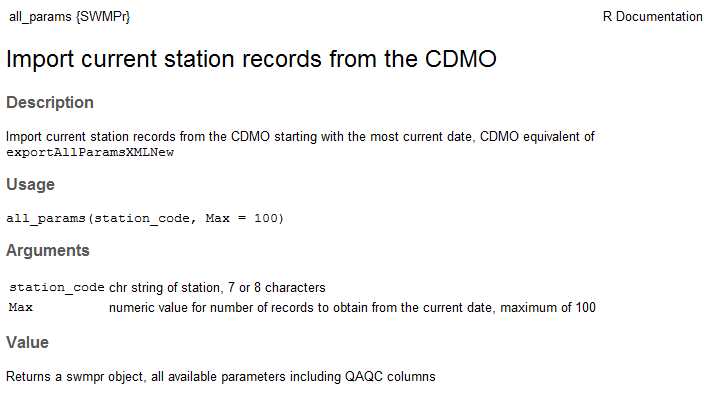
\includegraphics[width = 0.8\textwidth]{help_ex.png}}
\end{frame}

%%%%%%
\begin{frame}[fragile]{Overview of the SWMPr package}
Let's get some data into R!\\~\\
The \Bigtxt{retrieval} functions do two things: \\~\\
\begin{columns}[t]
\begin{column}{0.4\textwidth}
Import data directly from the CDMO:
\begin{knitrout}
\definecolor{shadecolor}{rgb}{0.969, 0.969, 0.969}\color{fgcolor}\begin{kframe}
\begin{alltt}
\hlstd{all_params}
\hlstd{all_params_dtrng}
\hlstd{single_param}
\end{alltt}
\end{kframe}
\end{knitrout}
These functions require \href{http://cdmo.baruch.sc.edu/webservices.cfm}{registering your IP address}  with CDMO, data are also rate-limited
\end{column}
\begin{column}{0.4\textwidth}
Import data from a local path:
\begin{knitrout}
\definecolor{shadecolor}{rgb}{0.969, 0.969, 0.969}\color{fgcolor}\begin{kframe}
\begin{alltt}
\hlstd{import_local}
\end{alltt}
\end{kframe}
\end{knitrout}
Allows import of data obtained from the \href{http://cdmo.baruch.sc.edu/aqs/zips.cfm}{zip downloads} feature
\end{column}
\end{columns}
\end{frame}

%%%%%%
\begin{frame}{Overview of the SWMPr package}
After unzipping, data from \href{http://cdmo.baruch.sc.edu/aqs/zips.cfm}{zip downloads} will have separate .csv files for each station and year\\~\\
\centerline{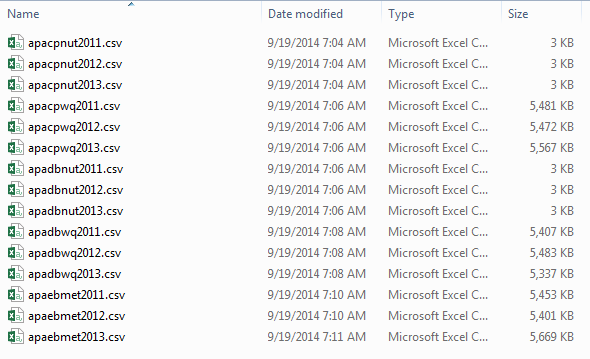
\includegraphics[width = 0.8\textwidth]{zips_ex.png}}
\end{frame}

%%%%%%
\begin{frame}[fragile]{Overview of the SWMPr package}
Use the following to import data into R:\\~\\
\begin{knitrout}
\definecolor{shadecolor}{rgb}{0.969, 0.969, 0.969}\color{fgcolor}\begin{kframe}
\begin{alltt}
\hlcom{# get data for apacpwq, all years}

\hlcom{# location of data}
\hlcom{# mypath <- 'C:/data/dataset1'}
\hlstd{mypath} \hlkwb{<-} \hlkwd{system.file}\hlstd{(}\hlstr{'zip_ex'}\hlstd{,} \hlkwc{package} \hlstd{=} \hlstr{'SWMPr'}\hlstd{)}

\hlcom{# import and assign to 'dat'}
\hlstd{dat} \hlkwb{<-} \hlkwd{import_local}\hlstd{(mypath,} \hlstr{'apacpwq'}\hlstd{,} \hlkwc{trace} \hlstd{= T)}
\end{alltt}
\end{kframe}
\end{knitrout}
\end{frame}

%%%%%%
\begin{frame}[fragile]{Overview of the SWMPr package}
Your console should look something like this:\\~\\
\begin{knitrout}
\definecolor{shadecolor}{rgb}{0.969, 0.969, 0.969}\color{fgcolor}\begin{kframe}
\begin{alltt}
\hlcom{# get data for apacpwq, all years}

\hlcom{# location of data}
\hlcom{# mypath <- 'C:/data/dataset1'}
\hlstd{mypath} \hlkwb{<-} \hlkwd{system.file}\hlstd{(}\hlstr{'zip_ex'}\hlstd{,} \hlkwc{package} \hlstd{=} \hlstr{'SWMPr'}\hlstd{)}

\hlcom{# import and assign to 'dat'}
\hlstd{dat} \hlkwb{<-} \hlkwd{import_local}\hlstd{(mypath,} \hlstr{'apacpwq'}\hlstd{,} \hlkwc{trace} \hlstd{= T)}
\end{alltt}
\begin{verbatim}
## Loading files...
## 
## apacpwq2011.csv 	apacpwq2012.csv 	apacpwq2013.csv 	
## 
## Combining data...
## 
## Data imported...
\end{verbatim}
\end{kframe}
\end{knitrout}
\end{frame}

%%%%%%
\begin{frame}[fragile, shrink]{Overview of the SWMPr package}
Now we have data in our `workspace' that we can organize/analyze

\begin{knitrout}\scriptsize
\definecolor{shadecolor}{rgb}{0.969, 0.969, 0.969}\color{fgcolor}\begin{kframe}
\begin{alltt}
\hlkwd{head}\hlstd{(dat)}
\end{alltt}
\begin{verbatim}
##         datetimestamp temp f_temp spcond f_spcond sal f_sal do_pct f_do_pct
## 1 2011-01-01 00:00:00   11   <0>      44     <0>   28  <0>      68     <0> 
## 2 2011-01-01 00:15:00   11   <0>      44     <0>   28  <0>      68     <0> 
## 3 2011-01-01 00:30:00   11   <0>      44     <0>   28  <0>      68     <0> 
## 4 2011-01-01 00:45:00   11   <0>      44     <0>   28  <0>      68     <0> 
## 5 2011-01-01 01:00:00   11   <0>      44     <0>   29  <0>      68     <0> 
## 6 2011-01-01 01:15:00   11   <0>      44     <0>   29  <0>      67     <0> 
##   do_mgl f_do_mgl depth f_depth cdepth f_cdepth level f_level clevel f_clevel
## 1      6     <0>      2    <0>       2     <3>     NA   <-1>      NA       NA
## 2      6     <0>      2    <0>       2     <3>     NA   <-1>      NA       NA
## 3      6     <0>      2    <0>       2     <3>     NA   <-1>      NA       NA
## 4      6     <0>      2    <0>       2     <3>     NA   <-1>      NA       NA
## 5      6     <0>      2    <0>       2     <3>     NA   <-1>      NA       NA
## 6      6     <0>      2    <0>       2     <3>     NA   <-1>      NA       NA
##   ph f_ph turb f_turb chlfluor f_chlfluor
## 1  8 <0>     3   <0>        NA      <-1> 
## 2  8 <0>     3   <0>        NA      <-1> 
## 3  8 <0>     2   <0>        NA      <-1> 
## 4  8 <0>     1   <0>        NA      <-1> 
## 5  8 <0>     2   <0>        NA      <-1> 
## 6  8 <0>     1   <0>        NA      <-1>
\end{verbatim}
\end{kframe}
\end{knitrout}
\end{frame}

%%%%%%
\begin{frame}
\vspace{0.3in}
\centerline{
\begin{tikzpicture}
  \node[drop shadow={shadow xshift=0ex,shadow yshift=0ex},fill=white,draw] at (0,0) {
\includegraphics[width=0.9\textwidth]{bg_main.jpg}};
\end{tikzpicture}}
\vspace{0.5in}
\Large
\centerline{\Bigtxt{Questions??}}
\end{frame}

\end{document}
